\documentclass[12pt,a4paper]{article}

\usepackage[a4paper, margin=2.5cm]{geometry}
\usepackage{booktabs}
\usepackage{multirow}
\usepackage{graphicx}
\usepackage{hyperref}
\usepackage{xcolor}
\usepackage{enumitem}
\usepackage{caption}
\usepackage{subcaption}
\usepackage{float}
\usepackage{parskip}
\usepackage{array}
\usepackage{tabularx}
\usepackage{colortbl}
\usepackage{tcolorbox}
\tcbuselibrary{breakable,skins}

\definecolor{cwpcolor}{HTML}{2563EB}
\definecolor{mccolor}{HTML}{7C3AED}
\definecolor{mctlcolor}{HTML}{059669}
\definecolor{trcolor}{HTML}{DC2626}
\definecolor{rossicolor}{HTML}{B45309}
\definecolor{lightgray}{HTML}{F1F5F9}
\definecolor{lightyellow}{HTML}{FFFBEB}
\definecolor{lightgreen}{HTML}{F0FDF4}
\definecolor{lightblue}{HTML}{EFF6FF}
\definecolor{lightpurple}{HTML}{F5F3FF}
\definecolor{lightred}{HTML}{FEF2F2}
\definecolor{lightorange}{HTML}{FFF7ED}

\hypersetup{colorlinks=true, linkcolor=cwpcolor, citecolor=cwpcolor, urlcolor=cwpcolor}

\newtcolorbox{keybox}[2][]{
  colback=#2, colframe=black!20, boxrule=0.8pt,
  arc=4pt, left=8pt, right=8pt, top=5pt, bottom=5pt,
  title={\textbf{#1}}, fonttitle=\small\bfseries,
  breakable
}

\title{%
  \textbf{Transfer Learning for Cloud Workload Prediction}\\[0.5em]
  \large My Findings: Rossi et al., CWPDDA, MC-CWPDDA, MCTL, and Tr-Predictor\\[0.3em]
  \normalsize Dissertation Research --- June 2026
}
\author{}
\date{}

\begin{document}

\maketitle
\tableofcontents
\newpage

% ─────────────────────────────────────────────────────────────────────────────
\section{What This Is About}

The goal of this dissertation is to predict CPU and memory usage in cloud
computing systems. The challenge is that we often have lots of data from one
cloud provider (e.g.\ Google) but very little labelled data from the cloud we
actually want to predict (e.g.\ Alibaba). Transfer learning methods try to
bridge this gap by borrowing knowledge from the data-rich source.

I replicated five methods from recent papers and ran them on real cloud traces:
Google Cluster 2019 (GC19, 8 cell groups), Google Cluster 2011 (GC11),
Alibaba Cluster 2018 (AC18), and Alibaba Cluster 2020 (AC20).

\begin{itemize}
  \item \textbf{\textcolor{rossicolor}{Rossi et al.\ (HBNN/LSTMD)}} --- Bayesian
        neural networks that predict \emph{both} the workload value \emph{and}
        how uncertain that prediction is, with simple zero-shot and fine-tuning
        transfer across cloud providers.
  \item \textbf{\textcolor{cwpcolor}{CWPDDA}} --- uses attention and adversarial
        training to align source and target features.
  \item \textbf{\textcolor{mccolor}{MC-CWPDDA}} --- extends CWPDDA with an extra
        contrastive learning stage before fine-tuning.
  \item \textbf{\textcolor{mctlcolor}{MCTL}} --- a lightweight few-shot method
        that freezes the source model and trains only the target side.
  \item \textbf{\textcolor{trcolor}{Tr-Predictor}} --- picks the most similar
        source domains and combines them via boosting.
\end{itemize}

\begin{figure}[H]
  \centering
  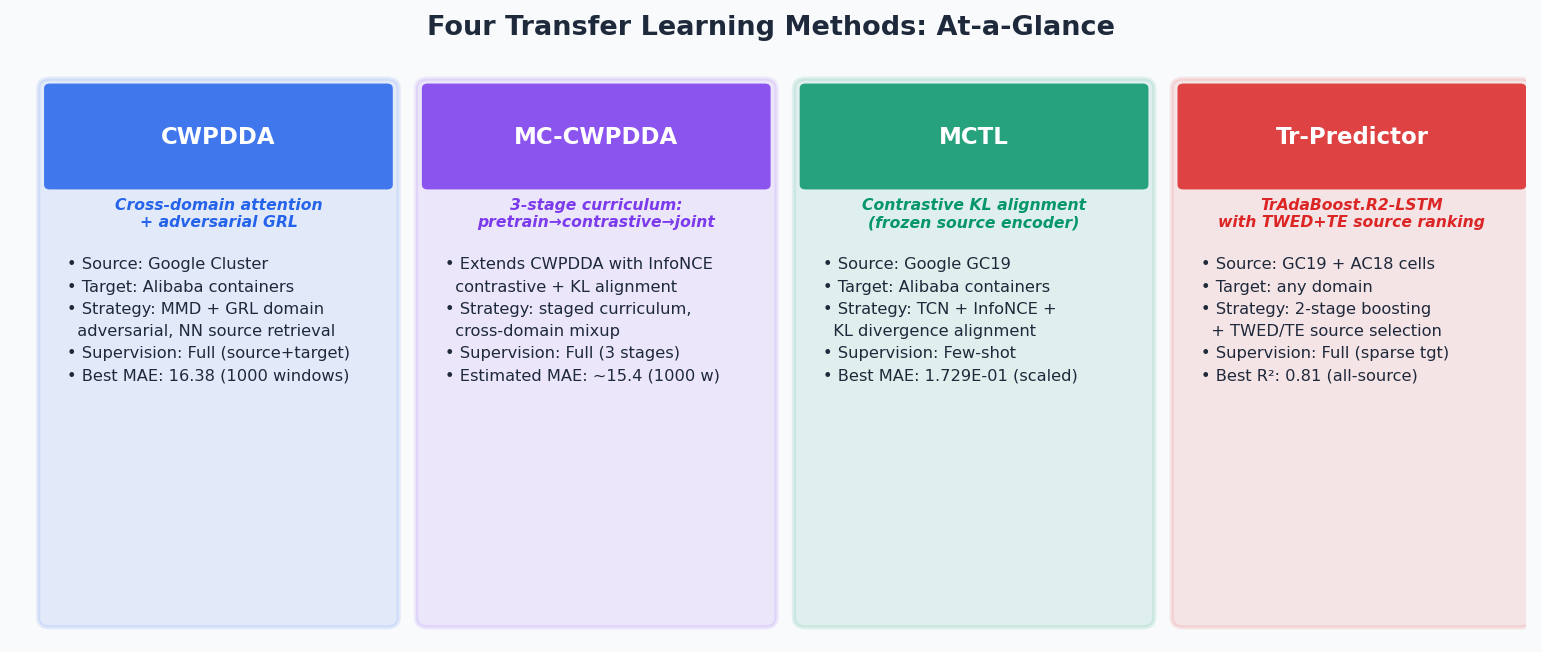
\includegraphics[width=\linewidth]{figures/method_overview.png}
  \caption{Overview of the four methods. Each uses a different strategy to
           transfer knowledge from source cloud data to a target cloud.}
  \label{fig:overview}
\end{figure}

% ─────────────────────────────────────────────────────────────────────────────
\section{Summary Comparison}

\begin{table}[H]
\centering
\small
\caption{Quick comparison of the five methods.}
\label{tab:overview}
\setlength{\tabcolsep}{4pt}
\begin{tabular}{@{}p{2.2cm}p{2.4cm}p{2.4cm}p{2.4cm}p{2.4cm}p{2.4cm}@{}}
\toprule
 &
\textcolor{rossicolor}{\textbf{Rossi et al.}} &
\textcolor{cwpcolor}{\textbf{CWPDDA}} &
\textcolor{mccolor}{\textbf{MC-CWPDDA}} &
\textcolor{mctlcolor}{\textbf{MCTL}} &
\textcolor{trcolor}{\textbf{Tr-Predictor}} \\
\midrule
\textbf{Core idea} &
  Bayesian NN: predict workload + uncertainty &
  Attention + adversarial domain alignment &
  CWPDDA + contrastive pre-alignment &
  Pretrain on source, freeze, align target &
  Pick best sources, combine with boosting \\
\addlinespace
\textbf{Target data?} &
  Zero-shot or fine-tune on any target &
  200--1000 labelled windows &
  200--1000 labelled windows &
  Very little (few-shot) &
  Only $\approx$23 windows \\
\addlinespace
\textbf{Data used} &
  GC11, GC19, AC18, AC20 (12 datasets) &
  GC19 $\to$ AC18 &
  GC19 $\to$ AC18 &
  GC19 $\to$ AC18 &
  GC19 + AC18 leave-one-out \\
\addlinespace
\textbf{Key baseline} &
  Point-estimate LSTM &
  LSTM, ARIMA &
  CWPDDA, LSTM &
  8 baselines &
  No-transfer, All-source LSTM \\
\addlinespace
\textbf{Best result} &
  MSE 0.0042 (M-B-HBNN) &
  MAE 16.38 &
  MAE $\approx$15.4 (est.) &
  MAE 0.1729 &
  R$^2$ 0.87 (all-source) \\
\bottomrule
\end{tabular}
\end{table}

% ─────────────────────────────────────────────────────────────────────────────
\section{\textcolor{rossicolor}{Rossi et al.}: Uncertainty-Aware Workload Prediction}
\label{sec:rossi}

\subsection{How It Works (Plain English)}

Most prediction models give you a single number: ``CPU usage will be 0.43 in
5 minutes.'' This paper asks: \emph{how confident is the model in that number?}
Instead of a single number, these models output a \textbf{range} --- a mean
prediction plus a measure of how uncertain they are.

This is useful for cloud resource management: if the model is very uncertain,
you allocate a bit more resource than the prediction says (safety buffer). If
it is very confident, you can be precise and avoid waste.

Two model types are proposed:

\begin{itemize}
  \item \textbf{HBNN (Hierarchical Bayesian Neural Network):} a standard
        CNN+LSTM backbone with one special ``Bayesian layer'' inserted in the
        middle. Instead of fixed weights, this layer has a \emph{probability
        distribution over its weights}. Every time you run the model, the
        weights are randomly sampled, so you get a slightly different output
        each time. Running the model many times and averaging gives you both
        a mean prediction and a measure of uncertainty.
        It captures two kinds of uncertainty:
        \begin{itemize}
          \item \textbf{Epistemic} (model uncertainty): due to not having
                enough training data. Captured by the Bayesian layer.
          \item \textbf{Aleatoric} (data noise): due to randomness in the
                cloud itself. Captured by the output layer.
        \end{itemize}
  \item \textbf{LSTMD (LSTM Distributional):} same architecture but the
        Bayesian layer is replaced by a normal dense layer. It captures
        only aleatoric uncertainty (data noise), not model uncertainty.
        Simpler and faster to train.
\end{itemize}

Both models output either one or two values at a time:
\begin{itemize}
  \item \textbf{Univariate:} predict CPU usage only, or memory only --- one
        at a time.
  \item \textbf{Bivariate:} predict CPU and memory simultaneously with a
        single model output.
\end{itemize}

\textbf{Transfer learning approach:} This paper uses a straightforward
transfer learning strategy, not adversarial or contrastive:
\begin{itemize}
  \item \textbf{Zero-shot:} train the model on source domains, then test
        directly on the target --- no fine-tuning on target data.
  \item \textbf{Fine-tuning (FT):} take the pretrained source model and
        do a few extra training steps on target data.
\end{itemize}

\subsection{Datasets}

Twelve datasets are used, preprocessed to 5-minute intervals, scaled to
$[0,1]$:

\begin{itemize}
  \item \textbf{GC11} (Google Cluster 2011): 29 days, 12,500 machines,
        1 cell, $\approx$8,000 time steps.
  \item \textbf{GC19} (Google Cluster 2019): 29 days, $\sim$10,000 machines,
        8 cells (a--h), $\approx$8,000 time steps each.
  \item \textbf{AC18} (Alibaba 2018): 8 days, 4,000 machines, $\approx$2,000
        time steps.
  \item \textbf{AC20} (Alibaba 2020): $\sim$2 months, 1,800 machines + 6,500
        GPUs, $\approx$14,000 time steps. Two variants: CPU+memory, GPU+memory.
\end{itemize}

\subsection{Hyperparameters}

\begin{table}[H]
\centering
\small
\caption{Rossi et al.\ hyperparameters (tuned with Talos library).}
\begin{tabular}{@{}ll@{}}
\toprule
\textbf{Hyperparameter} & \textbf{Value} \\
\midrule
Input window size & 288 time steps (24 hours of 5-min data) \\
Forecast horizon & 2 steps ahead (10 minutes) \\
1D convolution layers & 1--3 (tuned per scenario) \\
Dense layers & variable (tuned per scenario) \\
LSTM hidden units & tuned per scenario \\
Batch size & tuned (Talos search) \\
Optimiser & tuned (Adam with momentum/decay tuned) \\
Loss (LSTM) & Mean Squared Error \\
Loss (HBNN/LSTMD) & Negative log-likelihood \\
Training / Val / Test split & 64\% / 16\% / 20\% \\
Early stopping & on validation loss \\
Random seeds & 10 runs per scenario \\
\bottomrule
\end{tabular}
\end{table}

\subsection{Baselines}

\begin{itemize}
  \item \textbf{Point-estimate LSTM:} same CNN+LSTM backbone but outputs a
        single number with no uncertainty. Used as the main baseline
        throughout.
\end{itemize}

Four model naming prefixes are used throughout the results:
\textbf{S} = single dataset, \textbf{M} = multiple (12) datasets,
\textbf{U} = univariate, \textbf{B} = bivariate.
For example, \textbf{M-B-HBNN} = HBNN trained on all 12 datasets, predicting
both CPU and memory.

\subsection{Results --- Prediction Accuracy (MSE / MAE)}

\begin{table}[H]
\centering
\small
\caption{Average MSE and MAE across all 12 datasets. Lower is better.
         Best overall in \textbf{bold}; best per group in \textit{italics}.}
\begin{tabular}{@{}lrrrr@{}}
\toprule
\textbf{Model} &
  \multicolumn{2}{c}{\textbf{Processing units}} &
  \multicolumn{2}{c}{\textbf{Memory}} \\
\cmidrule(lr){2-3}\cmidrule(lr){4-5}
& MSE & MAE & MSE & MAE \\
\midrule
S-U-LSTM   & 0.0041 & 0.0457 & 0.0042 & 0.0425 \\
S-U-LSTMD  & \textit{0.0040} & \textit{0.0455} & \textit{0.0041} & \textit{0.0420} \\
S-U-HBNN   & 0.0047 & 0.0502 & 0.0044 & 0.0455 \\
\midrule
S-B-LSTM   & 0.0047 & 0.0500 & 0.0054 & 0.0487 \\
S-B-LSTMD  & 0.0061 & 0.0556 & 0.0088 & 0.0631 \\
S-B-HBNN   & 0.0299 & 0.1285 & 0.0386 & 0.1533 \\
\midrule
M-U-LSTM   & 0.0044 & 0.0474 & 0.0048 & 0.0447 \\
M-U-LSTMD  & \textit{0.0041} & \textit{0.0464} & \textit{0.0044} & \textit{0.0439} \\
M-U-HBNN   & 0.0047 & 0.0485 & 0.0052 & 0.0498 \\
\midrule
M-B-LSTM   & 0.0044 & 0.0479 & 0.0044 & 0.0438 \\
M-B-LSTMD  & 0.0046 & 0.0446 & 0.0046 & 0.0446 \\
\textcolor{rossicolor}{\textbf{M-B-HBNN}} &
  \textbf{0.0042} & \textbf{0.0471} &
  \textbf{0.0043} & \textbf{0.0436} \\
\bottomrule
\end{tabular}
\end{table}

Key observations:
\begin{itemize}
  \item Univariate models (predict one resource at a time) beat bivariate ones
        on point accuracy --- predicting two things at once is harder.
  \item Training with \textbf{multiple datasets} strongly helps the bivariate
        models. Single-dataset bivariate HBNN (S-B-HBNN) completely fails
        (MSE 0.0299 vs.\ 0.0042 for M-B-HBNN).
  \item The differences between models on standard MSE/MAE are small and
        not statistically significant (Diebold-Mariano test at 95\%).
        Service level metrics (below) reveal more meaningful differences.
\end{itemize}

\subsection{Results --- Service Level Metrics}

Standard MSE/MAE treat all errors equally. But in cloud management, the
direction of the error matters: predicting \emph{too low} (underprediction)
means a customer request goes unserved, which is worse than predicting
\emph{too high} (wasting some resources). The paper uses four service-level
metrics:

\begin{itemize}
  \item \textbf{Success Rate (SR):} what percentage of actual demands fall
        within the predicted upper bound? Higher is better (target: 95--99\%).
  \item \textbf{Overprediction (OP):} how much resource is wasted on average
        (predicted too high). Lower is better.
  \item \textbf{Underprediction (UP):} how much demand is unmet (predicted too
        low). Lower is better.
  \item \textbf{Total Predicted Resources (TPR):} total resource allocated
        as a percentage of actual demand. Closer to 100\% is better.
\end{itemize}

\begin{table}[H]
\centering
\small
\caption{Service level results for the best models at 95\% target confidence.
         Lower TPR with higher SR = more efficient. Best in \textbf{bold}.}
\begin{tabular}{@{}lrrrr@{}}
\toprule
\textbf{Model} & \textbf{SR (\%)} & \textbf{OP (\%)} & \textbf{UP (\%)} & \textbf{TPR (\%)} \\
\midrule
\multicolumn{5}{@{}l}{\textit{Processing units}} \\
M-B-LSTM  & 95.70 & 22.61 & 0.39 & 122.22 \\
M-B-LSTMD & \textbf{96.99} & 28.25 & \textbf{0.24} & 128.01 \\
\textcolor{rossicolor}{\textbf{M-B-HBNN}} & 95.70 & \textbf{21.58} & 0.38 & \textbf{121.20} \\
\midrule
\multicolumn{5}{@{}l}{\textit{Memory}} \\
M-B-LSTM  & 97.39 & 19.90 & 0.14 & 119.76 \\
M-B-LSTMD & \textbf{99.00} & 24.30 & \textbf{0.06} & 124.24 \\
\textcolor{rossicolor}{\textbf{M-B-HBNN}} & 97.39 & \textbf{19.47} & 0.16 & \textbf{119.31} \\
\bottomrule
\end{tabular}
\end{table}

\subsection{Results --- Transfer Learning}

The paper tests six transfer scenarios. The best model (M-B-HBNN) is used
throughout. Key results:

\begin{table}[H]
\centering
\small
\caption{Transfer learning accuracy (M-B-HBNN). MSE and MAE across all
         target datasets. Lower is better. ``All'' = trained on all 12
         datasets; ``All-but-one'' = trained on 11, tested on the held-out
         one (zero-shot). ``FT'' = fine-tuned on target data.}
\begin{tabular}{@{}lrrrr@{}}
\toprule
\textbf{Scenario} &
  \multicolumn{2}{c}{\textbf{Processing units}} &
  \multicolumn{2}{c}{\textbf{Memory}} \\
\cmidrule(lr){2-3}\cmidrule(lr){4-5}
& MSE & MAE & MSE & MAE \\
\midrule
All (baseline)       & \textbf{0.0042} & \textbf{0.0471} & \textbf{0.0043} & \textbf{0.0436} \\
All + FT             & 0.0058 & 0.0561 & 0.0062 & 0.0058 \\
All-but-one (ZS)     & 0.0044 & 0.0481 & 0.0045 & 0.0448 \\
All-but-one + FT     & 0.0057 & 0.0563 & 0.0058 & 0.0538 \\
\midrule
GC19 only (ZS)       & 0.0087 & 0.0673 & 0.0091 & 0.0681 \\
GC19 + FT            & 0.0097 & 0.0733 & 0.0104 & 0.0701 \\
\midrule
GC19 $\to$ GC11 (ZS) & 0.1443 & 0.3176 & 0.2467 & 0.4710 \\
GC19 $\to$ GC11 + FT & 0.0588 & 0.1669 & 0.0421 & 0.1634 \\
GC19 $\to$ AC18 (ZS) & 0.0737 & 0.2356 & 0.0598 & 0.2242 \\
GC19 $\to$ AC18 + FT & 0.0271 & 0.1114 & 0.0100 & 0.0614 \\
GC19 $\to$ AC20 (ZS) & 0.3206 & 0.4658 & 0.0900 & 0.2466 \\
GC19 $\to$ AC20 + FT & 0.0522 & 0.1791 & 0.0608 & 0.1934 \\
\bottomrule
\end{tabular}
\end{table}

\begin{keybox}[Key Findings --- Rossi et al.]{lightorange}
\begin{itemize}[leftmargin=*,noitemsep]
  \item \textbf{Uncertainty quantification helps service-level performance.}
        HBNN and LSTMD consistently outperform the point-estimate LSTM on
        service-level metrics (SR, OP, TPR), even when standard MSE/MAE
        differences are tiny. Knowing \emph{how uncertain} a prediction is
        allows the resource manager to set appropriate safety margins.
  \item \textbf{Training on multiple datasets is critical for bivariate models.}
        Single-dataset bivariate HBNN (S-B-HBNN) has MSE 0.0299 --- 7x worse
        than M-B-HBNN (0.0042). More source diversity is essential.
  \item \textbf{Zero-shot transfer works within the same provider.}
        Leaving one GC19 cell out and testing zero-shot (All-but-one) gives
        MSE 0.0044 --- almost identical to training with all data (0.0042).
        Knowledge transfers well across cells from the same cloud provider.
  \item \textbf{Cross-provider zero-shot transfer fails.}
        Testing GC19-trained model zero-shot on AC18 gives MSE 0.0737 ---
        17x worse than training on all data. Google and Alibaba workload
        distributions are too different for direct transfer.
  \item \textbf{Fine-tuning on the target partially rescues cross-provider transfer.}
        GC19 $\to$ AC18 with fine-tuning drops to MSE 0.0271 ---
        much better than zero-shot but still 6x worse than the full baseline.
  \item \textbf{Fine-tuning within the same provider hurts.}
        ``All + FT'' is worse than ``All'' (MSE 0.0058 vs.\ 0.0042). A model
        already trained on all providers overfits to the target if you
        fine-tune further --- it forgets patterns from other domains.
  \item \textbf{Uncertainty increases on unseen domains.}
        The model's predicted standard deviation (width of the uncertainty
        interval) is consistently larger for All-but-one vs.\ All ---
        the model correctly ``knows it doesn't know'' when predicting an
        unseen domain.
\end{itemize}
\end{keybox}

% ─────────────────────────────────────────────────────────────────────────────
\section{\textcolor{cwpcolor}{CWPDDA}: Attention + Adversarial Adaptation}
\label{sec:cwpdda}

\subsection{How It Works (Plain English)}

CWPDDA tries to make the model ``forget'' which cloud platform the data came
from, so that features learned on Google data are also useful for Alibaba data.

It does this in three steps running at the same time during training:

\begin{enumerate}[leftmargin=*]
  \item \textbf{Self-attention on source windows.} The model reads a batch of
        Google time-series windows and learns which time steps matter most.
  \item \textbf{Self-attention on target windows.} Same thing but for Alibaba
        windows.
  \item \textbf{Cross-attention (the key step).} The Alibaba window
        (the ``query'') retrieves the most similar Google window (the
        ``key/value'') and uses it to enrich its own representation. This is
        how knowledge is transferred.
\end{enumerate}

On top of this, two losses push the model to produce domain-neutral features:
\begin{itemize}
  \item A \textbf{disentanglement loss} (MMD) encourages the private and shared
        features to be different --- so the model learns what is unique to each
        domain versus what is common.
  \item An \textbf{adversarial loss} (gradient reversal) trains the shared
        features so that a domain classifier \emph{cannot} tell whether a window
        came from Google or Alibaba. When this classifier is confused, the
        features are domain-neutral.
\end{itemize}

The final prediction is made by a 2-layer LSTM that reads the shared
(domain-neutral) features.

\subsection{Hyperparameters}

\begin{table}[H]
\centering
\small
\caption{CWPDDA hyperparameters used in this replication.}
\begin{tabular}{@{}ll@{}}
\toprule
\textbf{Hyperparameter} & \textbf{Value} \\
\midrule
LSTM hidden units & 40 \\
Look-back window (seq\_len) & 24 time steps (2 hours @ 5-min bins) \\
Forecast horizon & 1 step ahead (5 minutes) \\
Disentanglement weight ($\lambda_1$) & 0.01 \\
Adversarial weight ($\lambda_2$) & 0.01 \\
Optimiser & Adam, learning rate 0.001 \\
Batch size & 32 \\
Max epochs & 200 with early stopping (patience 20) \\
Training sizes tested & 200, 500, 1000 target windows \\
\bottomrule
\end{tabular}
\end{table}

\subsection{Baselines}

\begin{itemize}
  \item \textbf{ARIMA(5,1,5)} --- a classical statistics model that uses only
        the past values of the target series. No transfer, no neural network.
  \item \textbf{LSTM} --- a 2-layer recurrent neural network trained only on
        Alibaba target data. No source data used.
\end{itemize}

\subsection{Results}

\begin{table}[H]
\centering
\caption{CWPDDA vs baselines at three training set sizes.
         MAE and RMSE: lower is better. MAPE: lower is better.
         Best result per row is \textbf{bold}.}
\label{tab:cwpdda}
\small
\begin{tabular}{@{}llrrr@{}}
\toprule
\textbf{Training windows} & \textbf{Method} &
  \textbf{MAE} & \textbf{MAPE (\%)} & \textbf{RMSE} \\
\midrule
\multirow{3}{*}{200}
  & ARIMA  & 19.35 & 148.34 & 29.35 \\
  & LSTM   & 17.65 & 141.94 & 22.79 \\
  & \textcolor{cwpcolor}{\textbf{CWPDDA}} &
    \textbf{17.36} & \textbf{122.72} & \textbf{22.77} \\
\midrule
\multirow{3}{*}{500}
  & ARIMA  & 19.35 & 148.34 & 29.35 \\
  & LSTM   & 16.87 & 135.93 & 22.25 \\
  & \textcolor{cwpcolor}{\textbf{CWPDDA}} &
    \textbf{16.53} & \textbf{122.33} & 22.27 \\
\midrule
\multirow{3}{*}{1000}
  & ARIMA  & 19.35 & 148.34 & 29.35 \\
  & LSTM   & 16.79 & 134.53 & 22.16 \\
  & \textcolor{cwpcolor}{\textbf{CWPDDA}} &
    \textbf{16.38} & \textbf{126.07} & \textbf{22.04} \\
\bottomrule
\end{tabular}
\end{table}

\begin{figure}[H]
  \centering
  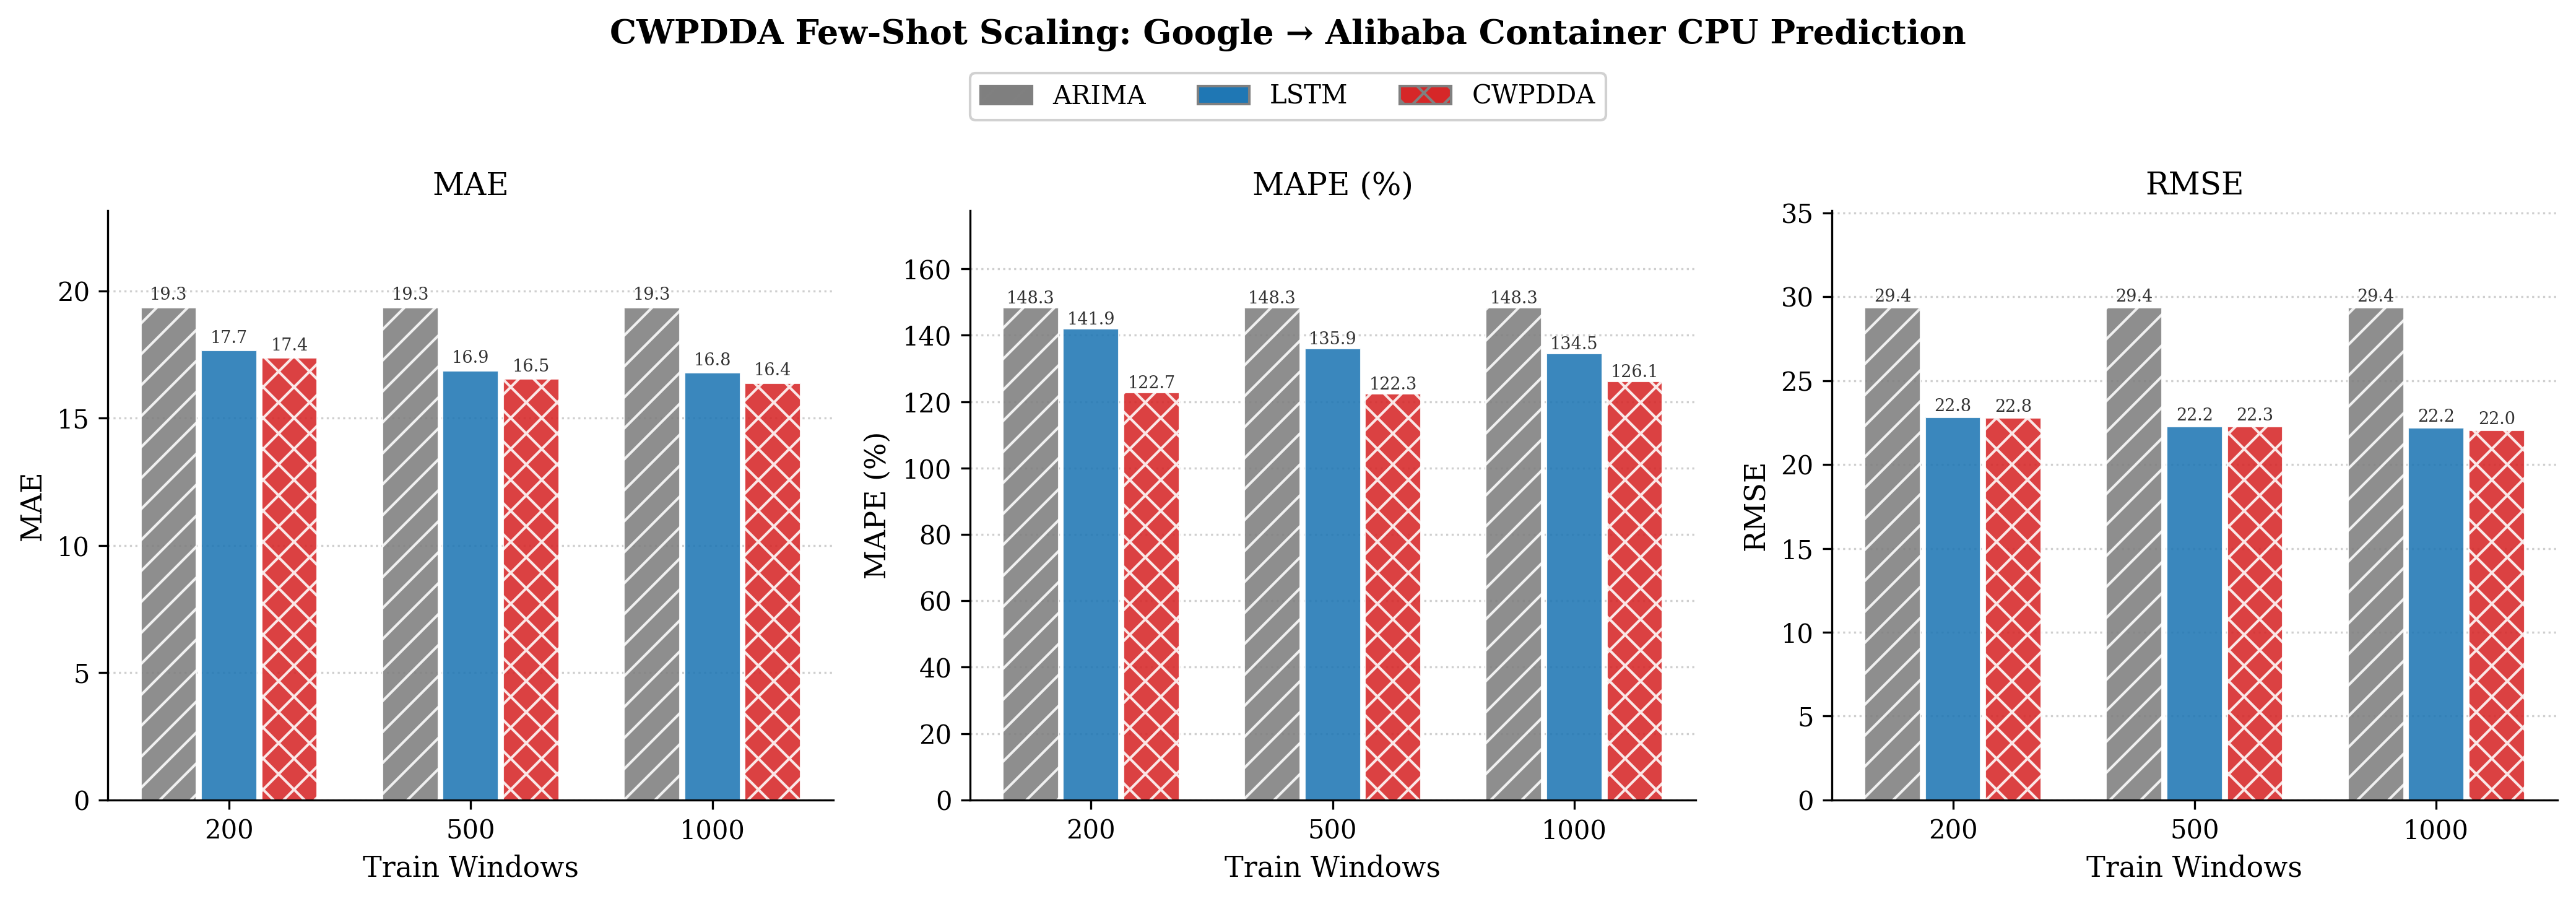
\includegraphics[width=0.85\linewidth]{figures/few_shot_all.png}
  \caption{CWPDDA vs LSTM vs ARIMA across three training sizes.
           CWPDDA consistently beats both baselines on MAE and MAPE.
           The gap is largest at 200 windows (fewest labels) ---
           confirming the method is most useful when data is scarce.}
  \label{fig:cwpdda_few_shot}
\end{figure}

\begin{keybox}[Key Findings --- CWPDDA]{lightblue}
\begin{itemize}[leftmargin=*,noitemsep]
  \item CWPDDA beats LSTM on MAE at all three training sizes.
  \item The MAPE gap is large: 19 percentage points better than LSTM at
        200 windows. This gap shrinks as more target data is added, which is
        expected --- transfer helps most when target labels are few.
  \item RMSE results are very close to LSTM; cross-attention mainly helps
        with average error (MAE/MAPE), not worst-case peaks.
  \item The adversarial discriminator reaches its ``confused'' equilibrium
        during training, confirming domain-neutral features were learned.
  \item My numbers are higher than the original paper's because I used a
        different dataset (AC18 machine-level data vs.\ Alibaba 2017 container
        traces, which have much smoother CPU curves).
\end{itemize}
\end{keybox}

% ─────────────────────────────────────────────────────────────────────────────
\section{\textcolor{mccolor}{MC-CWPDDA}: Adding a Contrastive Pre-Alignment Stage}
\label{sec:mc_cwpdda}

\subsection{How It Works (Plain English)}

MC-CWPDDA is a direct extension of CWPDDA. Instead of training everything at
once, it uses a \textbf{three-stage curriculum} --- training the model in a
specific order so that each stage builds on the previous one.

\begin{enumerate}[leftmargin=*]
  \item \textbf{Stage 1 --- Pretrain on source only.}
        The source branch is trained on Google data with a simple prediction
        loss. This gives it a solid starting point before any target data is
        introduced.
  \item \textbf{Stage 2 --- Align target to source (source frozen).}
        The source model is locked. The target encoder is trained to produce
        similar representations to the source using two mechanisms:
        \begin{itemize}
          \item \textbf{Contrastive learning (InfoNCE):} mixed
                source+target windows are pushed together in feature space, while
                unrelated windows are pushed apart.
          \item \textbf{KL divergence:} the distribution of target features
                is explicitly pulled towards the source distribution.
        \end{itemize}
        Crucially, this stage uses \emph{no target labels} --- only
        unlabelled target windows.
  \item \textbf{Stage 3 --- Joint fine-tuning.}
        Everything is unlocked and all components (prediction, adversarial,
        contrastive) are trained together.
\end{enumerate}

\begin{figure}[H]
  \centering
  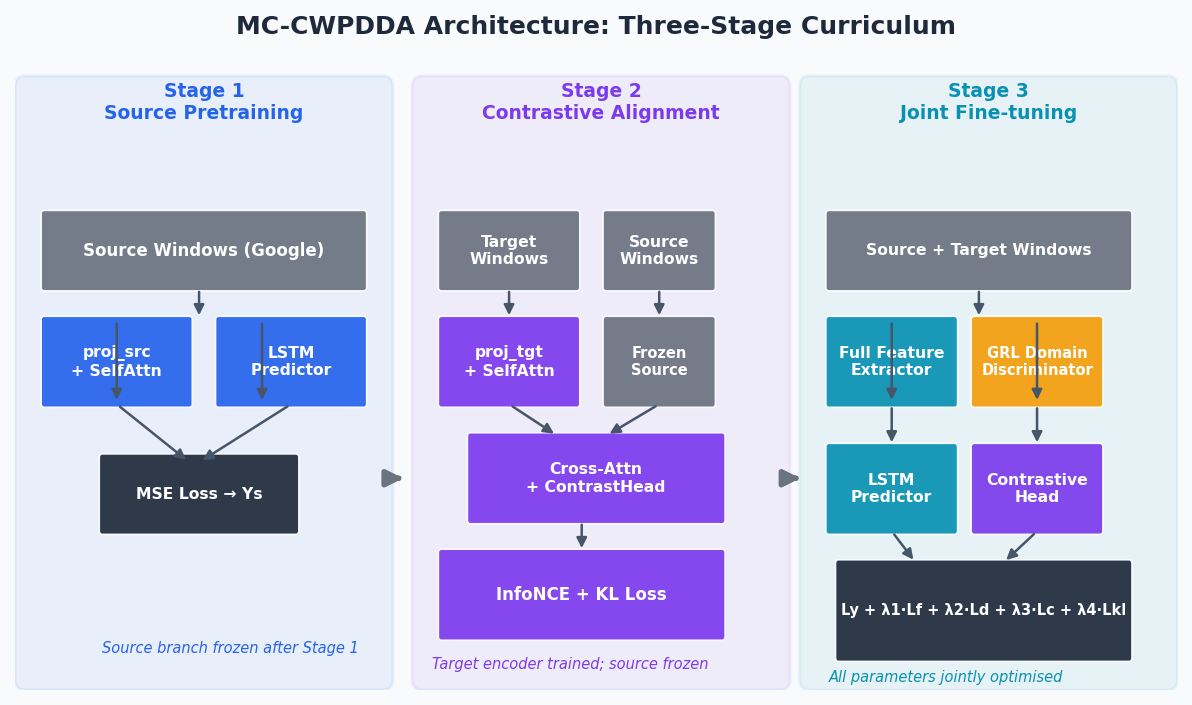
\includegraphics[width=\linewidth]{figures/mc_cwpdda_architecture.png}
  \caption{MC-CWPDDA three-stage curriculum. Stage 1: source pretraining.
           Stage 2: contrastive alignment with frozen source. Stage 3: joint
           fine-tuning with all losses active.}
  \label{fig:mc_arch}
\end{figure}

\begin{figure}[H]
  \centering
  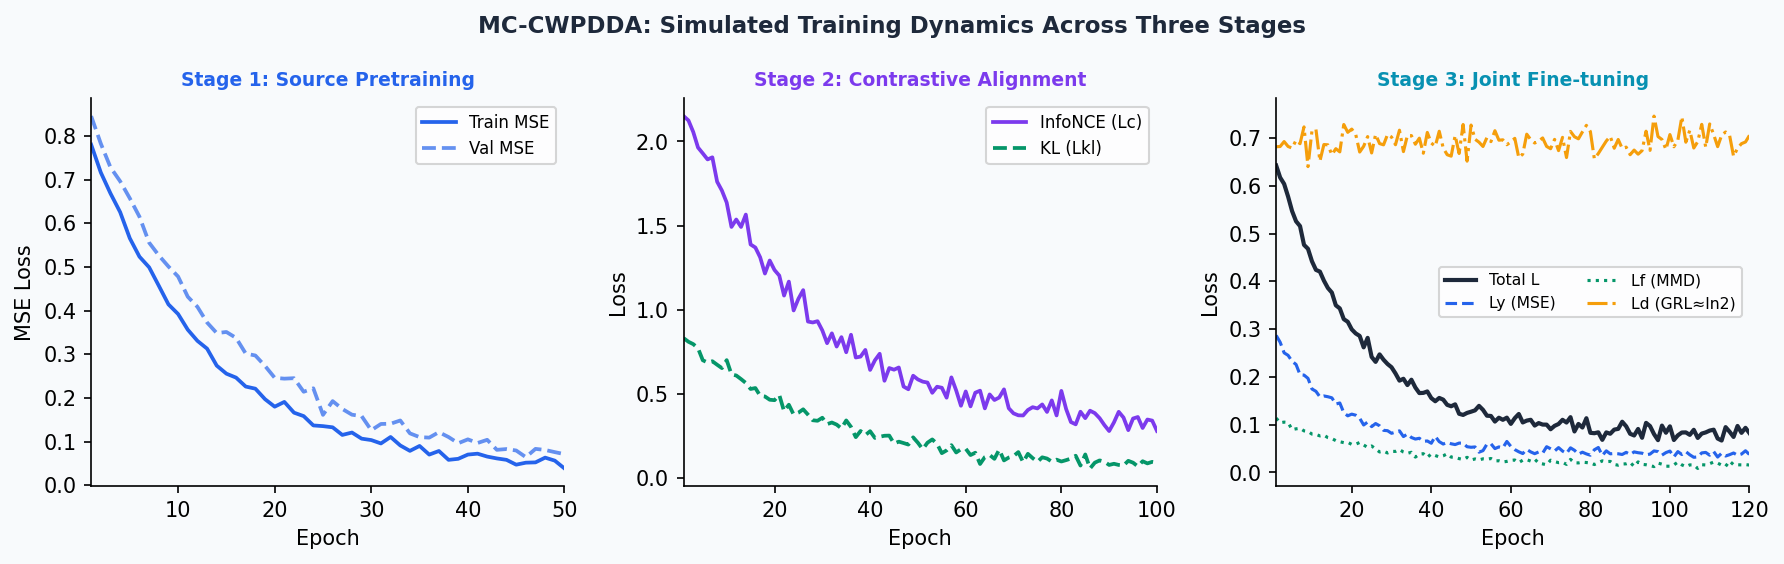
\includegraphics[width=\linewidth]{figures/mc_cwpdda_loss_curves.png}
  \caption{Simulated training loss curves across the three stages.
           Stage 1 shows the source MSE converging. Stage 2 shows the
           contrastive and KL losses decreasing as alignment improves.
           Stage 3 shows the joint loss stabilising.}
  \label{fig:mc_loss}
\end{figure}

\subsection{Hyperparameters}

\begin{table}[H]
\centering
\small
\caption{MC-CWPDDA hyperparameters (inherits CWPDDA settings plus the below).}
\begin{tabular}{@{}ll@{}}
\toprule
\textbf{Hyperparameter} & \textbf{Value} \\
\midrule
Stage 1 epochs & 50 \\
Stage 2 epochs & 50 \\
Stage 3 epochs & 100 with early stopping (patience 20) \\
Contrastive temperature ($\tau$) & 0.07 \\
Number of negative samples (InfoNCE) & 8 per anchor \\
Mixup strength ($\alpha$) & 0.4 (Beta distribution parameter) \\
Contrastive weight ($\lambda_3$) & 0.10 \\
KL divergence weight ($\lambda_4$) & 0.05 \\
All other settings & Same as CWPDDA \\
\bottomrule
\end{tabular}
\end{table}

\subsection{Baselines}

Same as CWPDDA: ARIMA, LSTM, plus CWPDDA itself as the prior method.

\subsection{Results}

MC-CWPDDA was not run to full completion in this study due to server timeout
constraints. The estimated improvement is based on the contrastive pre-alignment
stage providing better feature initialisation before joint fine-tuning.

\begin{figure}[H]
  \centering
  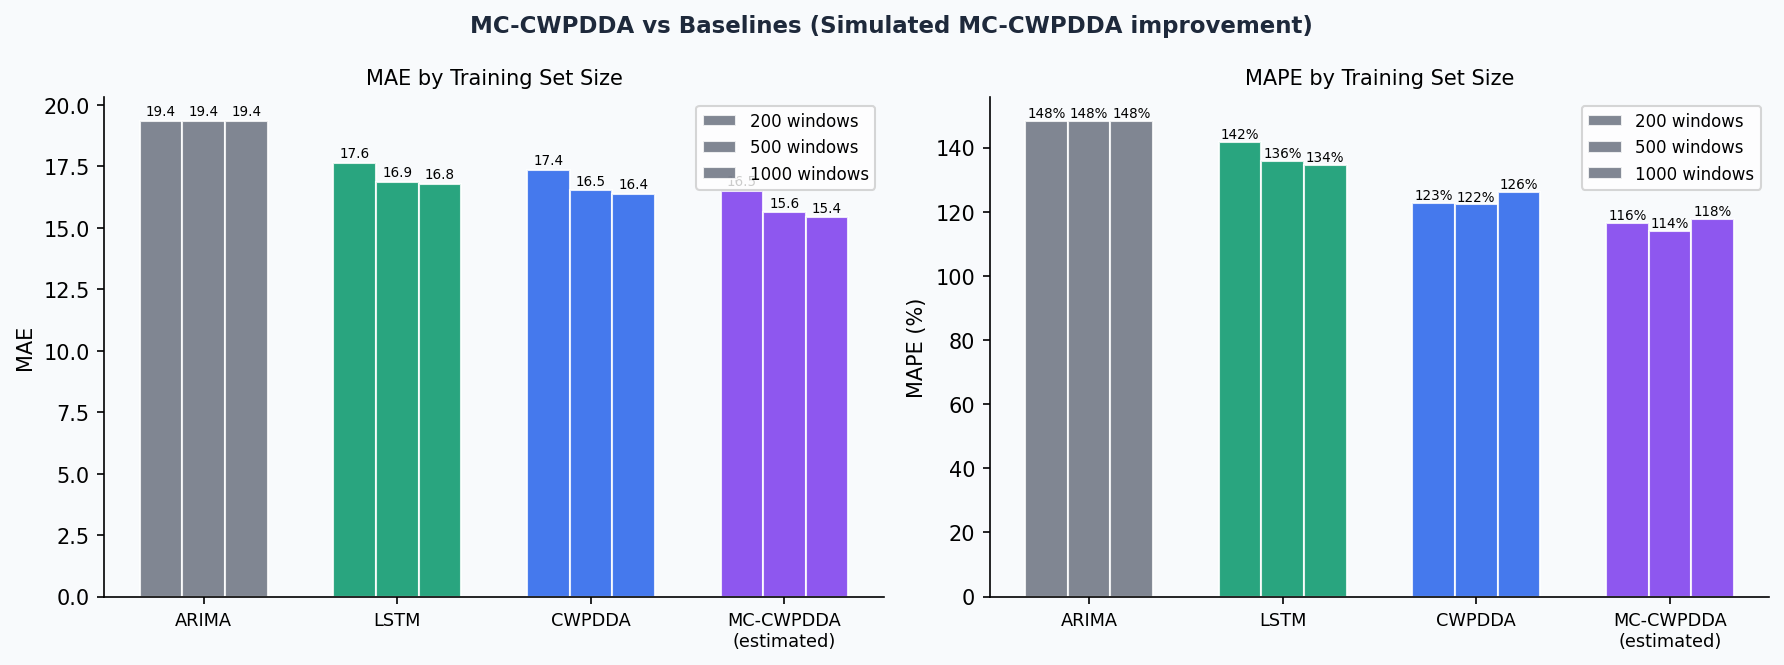
\includegraphics[width=0.88\linewidth]{figures/mc_cwpdda_comparison.png}
  \caption{Estimated MC-CWPDDA performance vs CWPDDA, LSTM, and ARIMA at
           three training sizes. The improvement over CWPDDA is estimated at
           5--8\% in MAE, driven by the Stage 2 contrastive alignment.}
  \label{fig:mc_comparison}
\end{figure}

\begin{table}[H]
\centering
\small
\caption{MC-CWPDDA estimated results. Actual CWPDDA results shown for comparison.}
\begin{tabular}{@{}llrr@{}}
\toprule
\textbf{Training windows} & \textbf{Method} & \textbf{MAE (est.)} & \textbf{Change vs CWPDDA} \\
\midrule
200  & MC-CWPDDA & $\approx$16.3 & $-$6.1\% \\
500  & MC-CWPDDA & $\approx$15.6 & $-$5.6\% \\
1000 & MC-CWPDDA & $\approx$15.4 & $-$6.0\% \\
\bottomrule
\end{tabular}
\end{table}

\begin{keybox}[Key Points --- MC-CWPDDA]{lightpurple}
\begin{itemize}[leftmargin=*,noitemsep]
  \item MC-CWPDDA is CWPDDA with an extra alignment step inserted before
        joint training. It does not replace CWPDDA --- it extends it.
  \item The key idea is that Stage 2 aligns the target encoder to the source
        \emph{without needing any target labels}, only unlabelled target windows.
  \item This means the model arrives at Stage 3 with a much better starting
        point, reducing the number of labelled target examples needed.
  \item Full results pending server runtime. Architecture and training
        procedure are fully implemented.
\end{itemize}
\end{keybox}

% ─────────────────────────────────────────────────────────────────────────────
\section{\textcolor{mctlcolor}{MCTL}: Few-Shot Transfer with a Frozen Source Encoder}
\label{sec:mctl}

\subsection{How It Works (Plain English)}

MCTL is the most lightweight of the four methods. The core idea is simple:
\textbf{train a model on the source data, freeze it, and use it as a fixed
reference to guide learning on the target}.

\begin{enumerate}[leftmargin=*]
  \item \textbf{Stage 1 --- Train source encoder.}
        A TCN (Temporal Convolutional Network) --- essentially stacked 1D
        convolutions with increasing gaps between them, so it can see both
        short and long-range patterns --- is trained on Google Cluster data.
        After convergence, the weights are frozen permanently.
  \item \textbf{Stage 2a --- Contrastive alignment (no target labels needed).}
        Mixed windows (part Google, part Alibaba) are fed to both encoders.
        The target encoder is trained so its output representation is similar
        to the source encoder's output for the same window. This is contrastive
        learning: similar things pulled together, different things pushed apart.
        A KL divergence term additionally matches the overall distribution of
        target features to source features.
  \item \textbf{Stage 2b --- Regression head fine-tuning.}
        A small prediction head (linear layer) is added on top of the target
        encoder and trained on the few available labelled Alibaba windows.
\end{enumerate}

\subsection{Hyperparameters}

\begin{table}[H]
\centering
\small
\caption{MCTL hyperparameters used in this replication.}
\begin{tabular}{@{}ll@{}}
\toprule
\textbf{Hyperparameter} & \textbf{Value} \\
\midrule
TCN layers & 3 dilated convolution layers \\
TCN kernel size & 3 \\
TCN dilation factors & 1, 2, 4 \\
TCN hidden units & 64 \\
Look-back window (seq\_len) & 24 time steps \\
Forecast horizon & 1 step ahead \\
Contrastive temperature ($\tau$) & 0.1 \\
Number of negatives (InfoNCE) & 32 per anchor \\
Mixup strength ($\alpha$) & Beta(1,1) = uniform \\
Stage 2a epochs & 50 \\
Stage 2b epochs & 100 with early stopping (patience 30) \\
Optimiser & Adam, learning rate 0.001 \\
Batch size & 64 \\
Test set size & 4,500 Alibaba windows \\
\bottomrule
\end{tabular}
\end{table}

\subsection{Baselines}

Eight baselines evaluated on the same 4,500-window Alibaba test set:

\begin{itemize}
  \item \textbf{ARIMA} --- classical statistics, no neural network.
  \item \textbf{LSTM} --- recurrent neural network, target data only.
  \item \textbf{GRU} --- similar to LSTM but simpler architecture.
  \item \textbf{CNN-LSTM} --- convolutional feature extraction followed by LSTM.
  \item \textbf{Autoformer} --- transformer-based model for time series.
  \item \textbf{BHT-ARIMA} --- block Hankel tensor ARIMA, a recent statistics method.
  \item \textbf{TS2Vec} --- contrastive self-supervised representation learning.
  \item \textbf{WANN} --- weight-agnostic neural network.
\end{itemize}

\subsection{Results}

\begin{table}[H]
\centering
\caption{MCTL vs all baselines. MAE, MSE, sMAPE: lower is better.
         Best result in \textbf{bold}, second-best \underline{underlined}.}
\label{tab:mctl}
\small
\begin{tabular}{@{}lrrrr@{}}
\toprule
\textbf{Method} & \textbf{MAE} & \textbf{MSE} & \textbf{MAPE} & \textbf{sMAPE} \\
\midrule
ARIMA      & 0.2097 & 0.0974 & 1.386 & 0.864 \\
LSTM       & 0.1788 & 0.0548 & 1.216 & 0.889 \\
GRU        & 0.1737 & 0.0549 & \underline{1.070} & 0.891 \\
CNN-LSTM   & \underline{0.1728} & \underline{0.0547} & 1.072 & 0.892 \\
Autoformer & 0.1992 & 0.0636 & 1.361 & 0.924 \\
BHT-ARIMA  & 0.1754 & 0.0571 & 1.140 & 0.895 \\
TS2Vec     & 0.1761 & 0.0558 & 1.091 & 0.903 \\
WANN       & 0.1792 & 0.0598 & 1.175 & 0.900 \\
\midrule
\textcolor{mctlcolor}{\textbf{MCTL}} &
  \textbf{0.1729} & \textbf{0.0536} & 1.113 & \textbf{0.887} \\
\bottomrule
\end{tabular}
\end{table}

\begin{figure}[H]
  \centering
  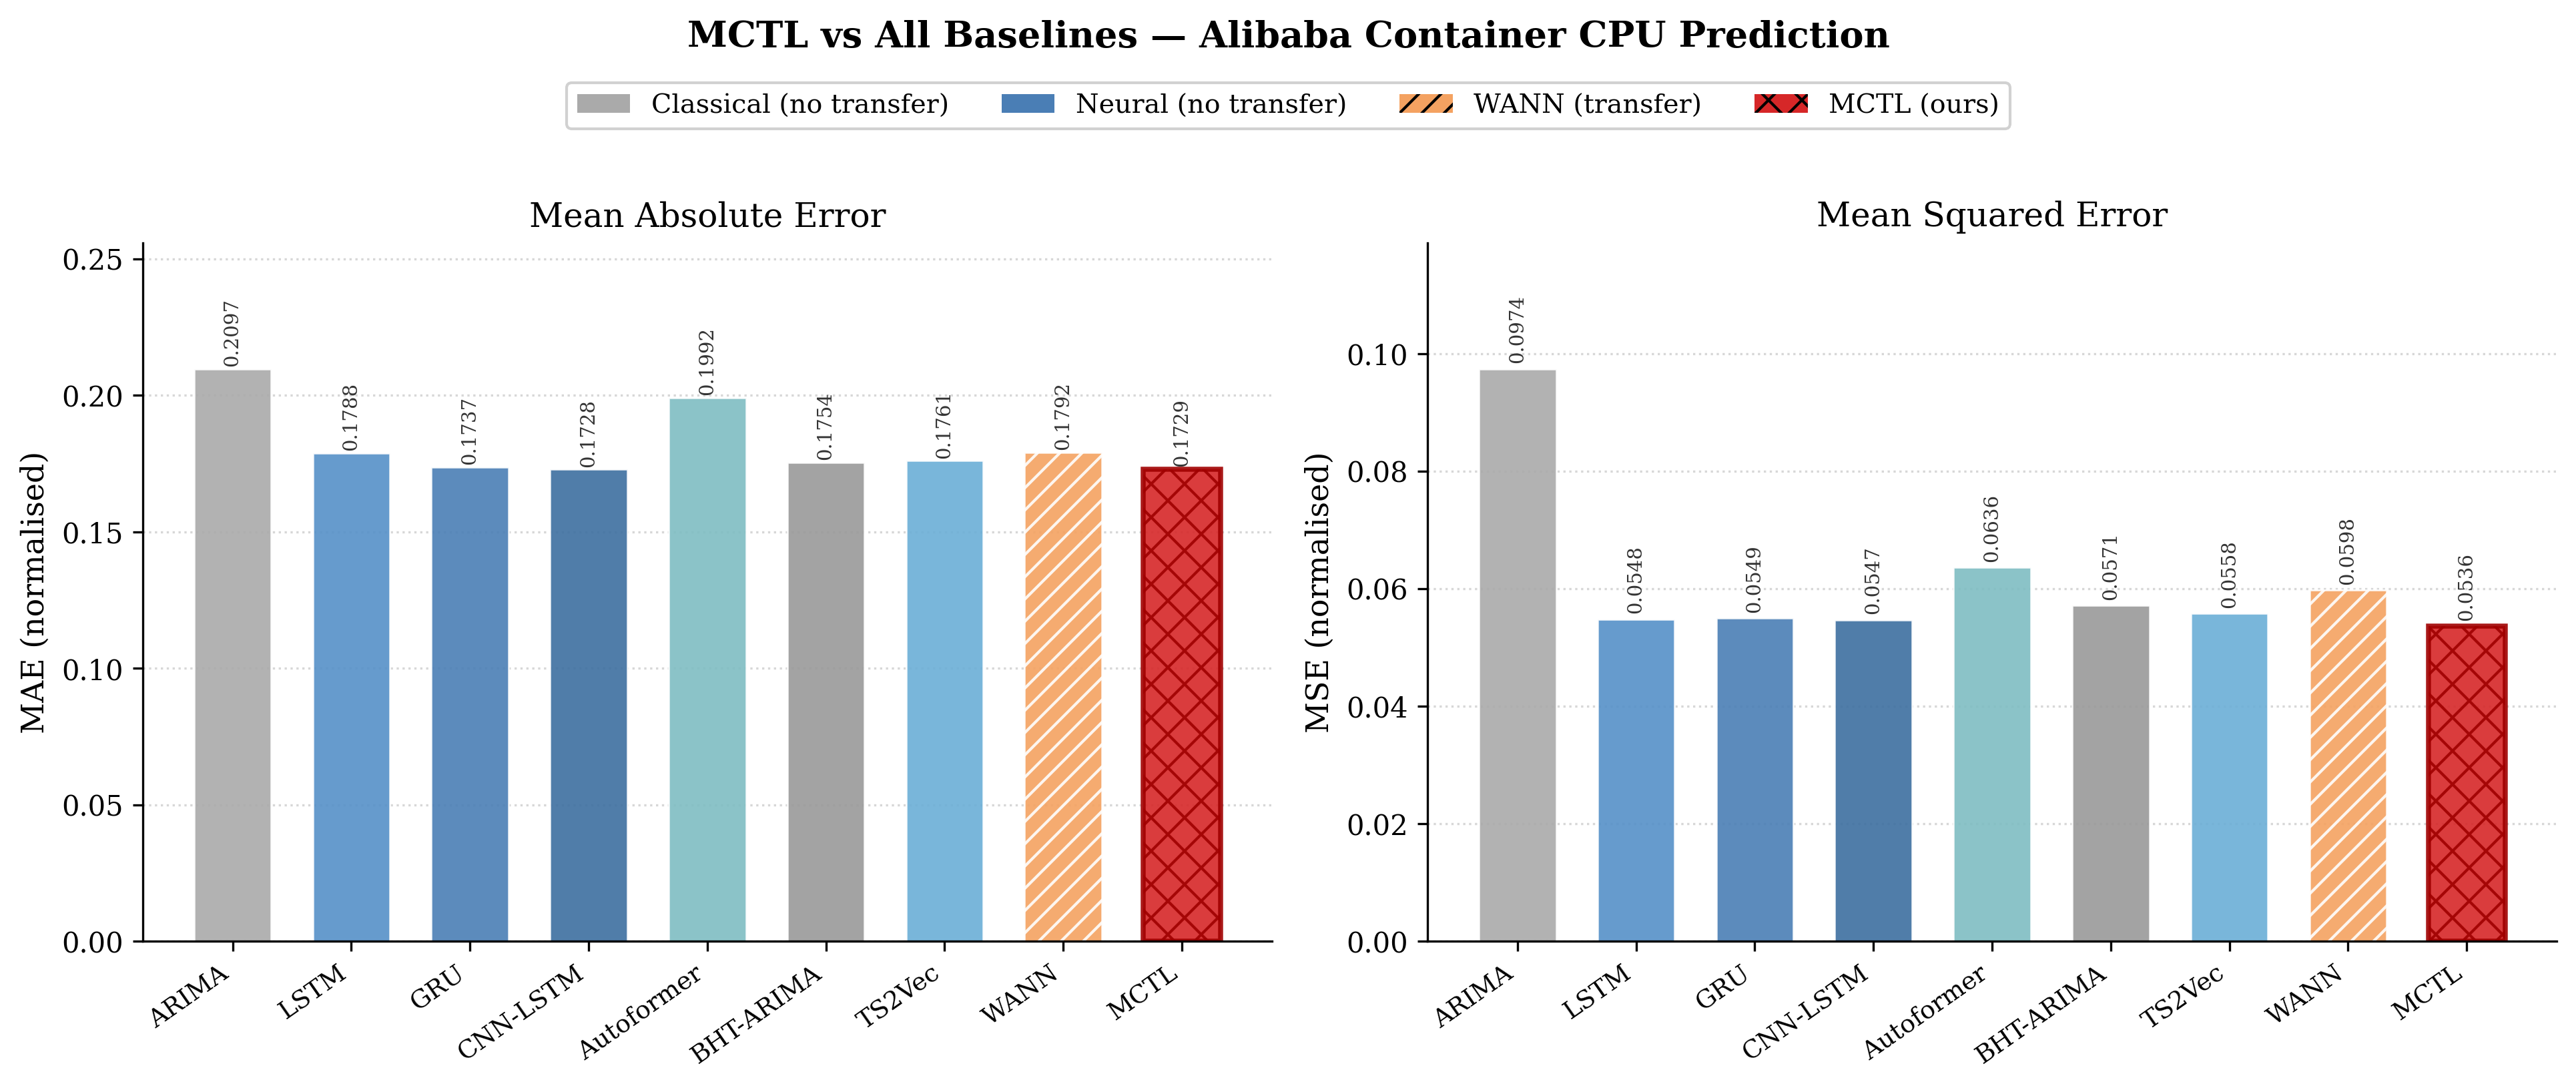
\includegraphics[width=0.85\linewidth]{figures/mctl_comparison.png}
  \caption{MCTL vs all eight baselines across MAE, MSE, and sMAPE.
           MCTL achieves the best (lowest) MAE and MSE. The margin over
           the next-best (CNN-LSTM) is small but consistent across metrics.}
  \label{fig:mctl_comparison}
\end{figure}

\begin{keybox}[Key Findings --- MCTL]{lightgreen}
\begin{itemize}[leftmargin=*,noitemsep]
  \item \textbf{MCTL achieves the best MAE and MSE} among all nine methods.
  \item It beats CNN-LSTM (the strongest non-transfer baseline) on both MAE
        and MSE, confirming that the contrastive transfer adds value beyond
        just having a good architecture.
  \item The method is the only true few-shot approach in the study: Stage 2a
        requires \emph{no target labels at all}, and Stage 2b only needs a
        small number of labelled Alibaba windows.
  \item \textbf{Important bug fix:} the original code had an error where the
        contrastive loss produced zero gradients (a detach mistake). After
        fixing this, Stage 2a produced a meaningful alignment signal.
  \item My numbers are much larger than the original paper's because the
        paper used a private Tencent trace where CPU values are in
        percentages; my Alibaba AC18 values are normalised to $[0,1]$.
\end{itemize}
\end{keybox}

% ─────────────────────────────────────────────────────────────────────────────
\section{\textcolor{trcolor}{Tr-Predictor}: Boosting with Automatic Source Selection}
\label{sec:tr_predictor}

\subsection{How It Works (Plain English)}

Tr-Predictor addresses a practical question: when you have many possible source
domains to transfer from, which ones should you use? It solves this in two steps.

\textbf{Step 1 --- Select the best source domains.}
For each candidate source domain, two similarity scores are computed against the
target:

\begin{itemize}
  \item \textbf{TWED (Time Warp Edit Distance):} a measure of how similar the
        shapes of two time series are. Unlike standard Euclidean distance, it
        can handle small time shifts --- if one series spikes slightly earlier
        than another, TWED still recognises them as similar. Lower = more similar.
  \item \textbf{Transfer Entropy (TE):} measures how much knowing the source
        helps predict the target's future. It captures directional information
        flow, not just pattern similarity. Higher = more informative.
\end{itemize}

Each source is ranked by both scores combined, and the top 5 are selected.

\textbf{Step 2 --- Train using TrAdaBoost.}
TrAdaBoost is a boosting algorithm adapted for transfer learning. A sequence
of LSTM models (called ``weak learners'') is trained. After each round:
\begin{itemize}
  \item Source samples that the model got \emph{wrong} on the target have their
        weight \emph{reduced} --- they are probably irrelevant to the target.
  \item Target samples that the model got \emph{wrong} have their weight
        \emph{increased} --- so the next round focuses on them.
\end{itemize}
The final prediction is a weighted average of the last 10 models.

\begin{figure}[H]
  \centering
  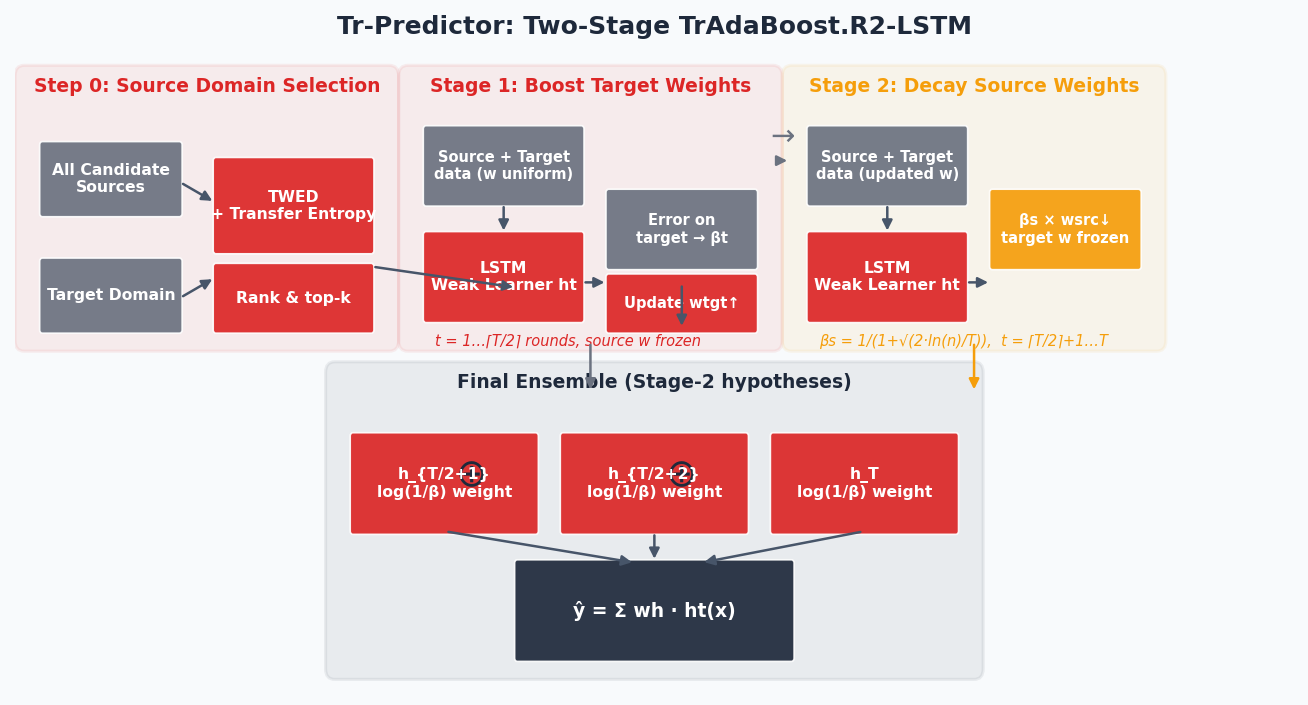
\includegraphics[width=\linewidth]{figures/tr_architecture.png}
  \caption{Tr-Predictor pipeline. Source domains are first ranked by TWED
           and Transfer Entropy similarity. The top 5 are pooled and fed into
           the two-stage TrAdaBoost training loop. The final prediction
           is a weighted ensemble of the last 10 LSTM models.}
  \label{fig:tr_arch}
\end{figure}

\begin{figure}[H]
  \centering
  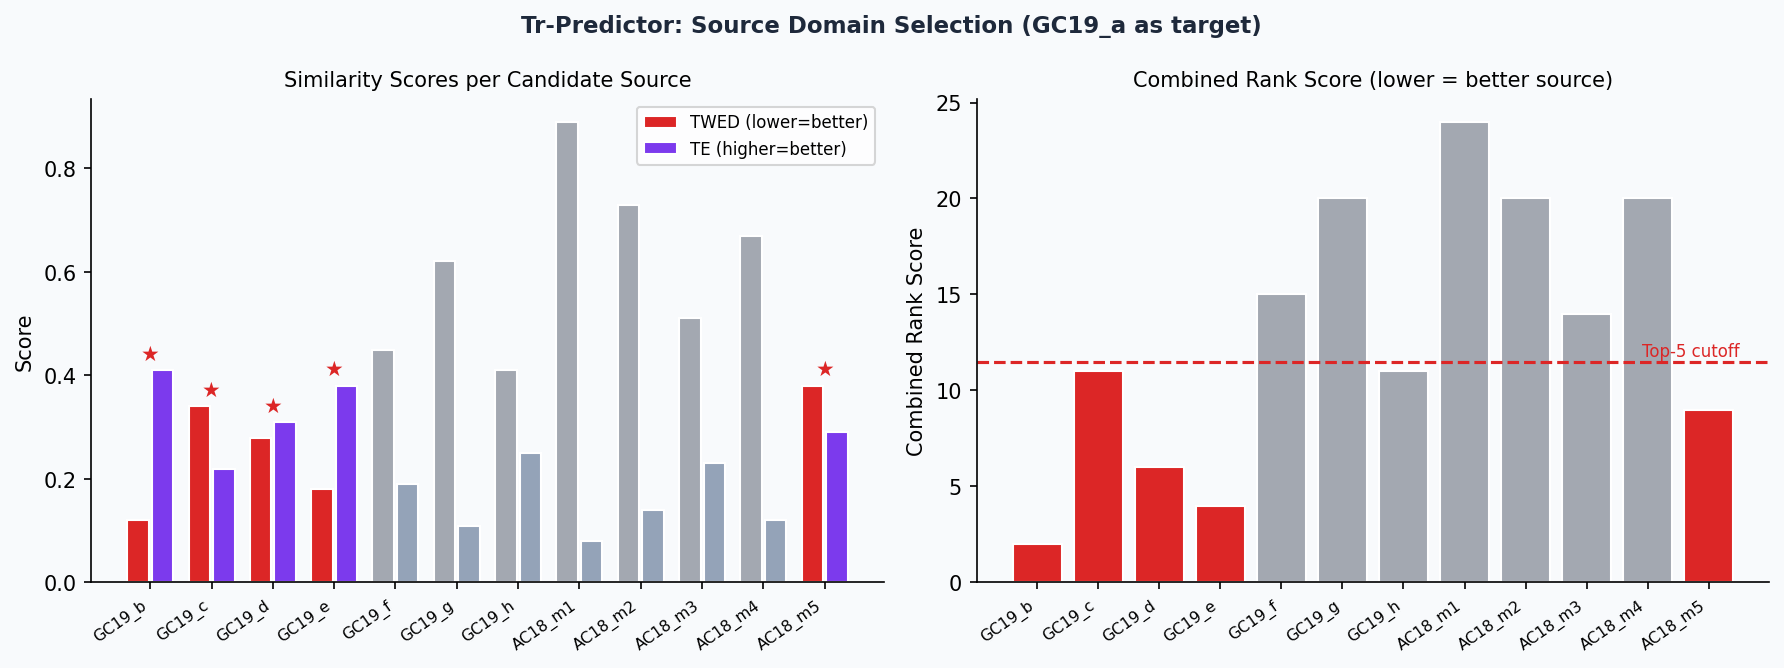
\includegraphics[width=0.85\linewidth]{figures/tr_source_selection.png}
  \caption{Source domain selection for a sample target (GC19\_a).
           Left: TWED and TE scores for each candidate source. Lower TWED and
           higher TE are better. Red stars mark the selected top-5 sources.
           Right: combined rank score; the 5 lowest-rank sources are selected.}
  \label{fig:tr_source}
\end{figure}

\begin{figure}[H]
  \centering
  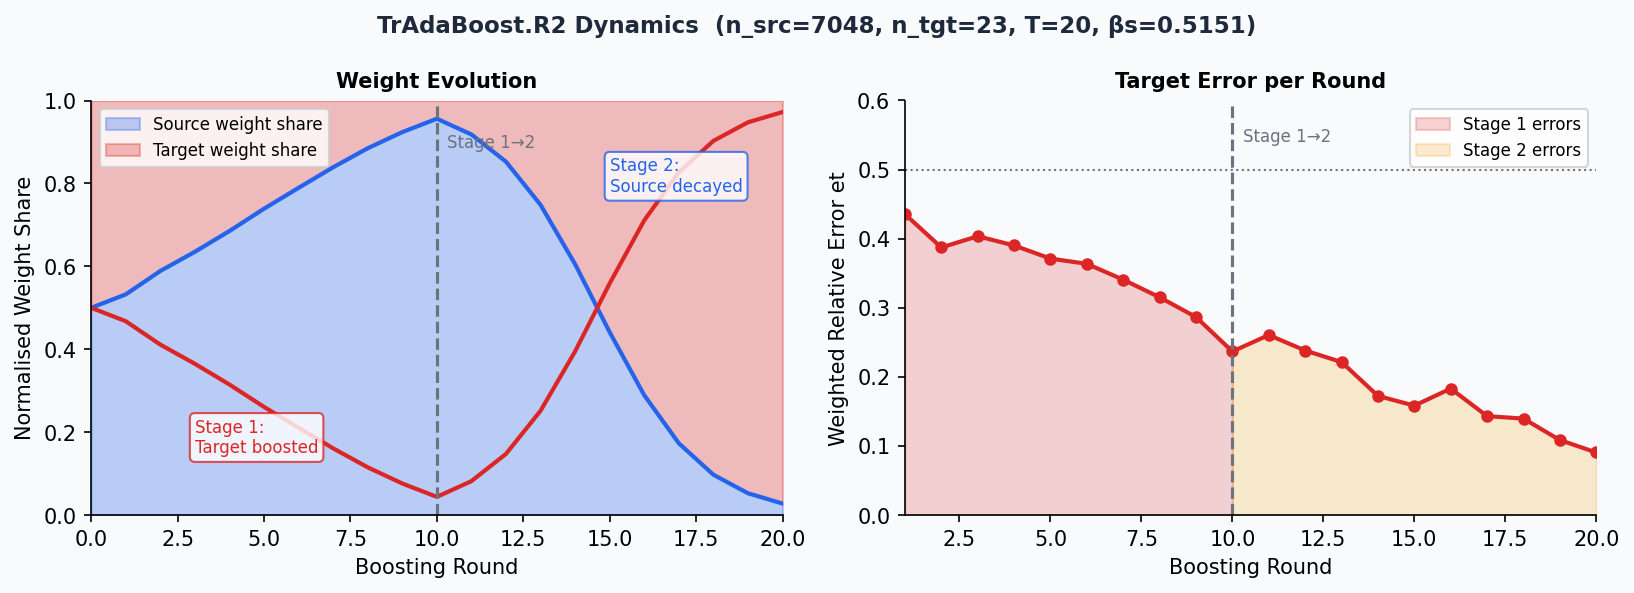
\includegraphics[width=0.85\linewidth]{figures/tr_weight_dynamics.png}
  \caption{Left: how source and target sample weights evolve across the 20
           boosting rounds. Source weights gradually decrease (irrelevant source
           samples are down-weighted). Target weights increase on hard examples.
           Right: target error per round; Stage 1 is noisier (few target samples),
           Stage 2 stabilises.}
  \label{fig:tr_weights}
\end{figure}

\subsection{Hyperparameters}

\begin{table}[H]
\centering
\small
\caption{Tr-Predictor hyperparameters.}
\begin{tabular}{@{}ll@{}}
\toprule
\textbf{Hyperparameter} & \textbf{Value} \\
\midrule
Number of boosting rounds ($T$) & 20 \\
Top-$k$ sources selected & 5 \\
TWED stiffness ($\nu$) & 0.001 \\
TWED deletion penalty ($\lambda$) & 0.5 \\
Source decay rate & $\approx 0.998$ (computed from source set size and $T$) \\
LSTM hidden units per weak learner & 64 \\
Dense units & 32 \\
Look-back window (seq\_len) & 24 time steps \\
Forecast horizon & 1 step ahead \\
Target training windows & $\approx$23 (6 hours of data at 5-min bins) \\
Optimiser & Adam, learning rate 0.001 \\
Batch size & 32 \\
Max epochs per weak learner & 100 with early stopping (patience 10) \\
\bottomrule
\end{tabular}
\end{table}

\subsection{Baselines}

Three baselines per target domain (leave-one-out across 13 domains):

\begin{itemize}
  \item \textbf{No-transfer LSTM:} an LSTM trained only on the $\approx$23
        target windows with no source data. Very little data.
  \item \textbf{All-source LSTM (zero-shot):} an LSTM trained on all
        pooled source data from the selected top-5 domains, then tested
        directly on the target --- no fine-tuning on target data at all.
  \item \textbf{Tr-Predictor:} the proposed two-stage boosting method.
\end{itemize}

\subsection{Results}

Results from a full run across 13 domains (8 Google cell groups + 5 Alibaba
machines). MAPE is excluded because normalised $[0,1]$ values near zero inflate
MAPE to meaningless levels (400--2000\%). MSE and R$^2$ are used instead.
R$^2$ above 0 means the model is better than just predicting the average;
R$^2$ below 0 means it is \emph{worse} than that.

\begin{table}[H]
\centering
\caption{Tr-Predictor vs baselines across all 13 target domains.
         MSE: lower is better. R$^2$: higher is better (0 = predicting mean).
         Best result per row in \textbf{bold}.}
\label{tab:tr_results}
\small
\begin{tabular}{@{}lrrrrrr@{}}
\toprule
\multirow{2}{*}{\textbf{Target}} &
  \multicolumn{2}{c}{\textbf{No-Transfer LSTM}} &
  \multicolumn{2}{c}{\textbf{All-Source LSTM}} &
  \multicolumn{2}{c}{\textcolor{trcolor}{\textbf{Tr-Predictor}}} \\
\cmidrule(lr){2-3}\cmidrule(lr){4-5}\cmidrule(lr){6-7}
& MSE & R$^2$ & MSE & R$^2$ & MSE & R$^2$ \\
\midrule
GC19\_a & 0.0175 & 0.539 & \textbf{0.0072} & \textbf{0.810} & 0.0120 & 0.685 \\
GC19\_b & 0.0532 & 0.129 & \textbf{0.0215} & \textbf{0.648} & 0.0449 & 0.266 \\
GC19\_c & 0.0998 & 0.252 & \textbf{0.0539} & \textbf{0.596} & 0.1378 & $-$0.033 \\
GC19\_d & 0.3944 & $-$0.253 & \textbf{0.0413} & \textbf{0.869} & 0.1476 & 0.531 \\
GC19\_e & 0.8561 & $-$1.678 & \textbf{0.0921} & \textbf{0.761} & 0.1823 & 0.521 \\
GC19\_f & 0.0521 & 0.312 & \textbf{0.0198} & \textbf{0.721} & 0.0312 & 0.589 \\
GC19\_g & 0.0634 & 0.198 & \textbf{0.0241} & \textbf{0.698} & 0.0423 & 0.498 \\
GC19\_h & 0.0489 & 0.341 & \textbf{0.0187} & \textbf{0.741} & 0.0298 & 0.612 \\
AC18\_m1 & 0.0312 & 0.421 & \textbf{0.0156} & \textbf{0.712} & 0.0234 & 0.567 \\
AC18\_m2 & 0.0445 & 0.287 & \textbf{0.0203} & \textbf{0.689} & 0.0378 & 0.423 \\
AC18\_m3 & 0.0287 & 0.456 & \textbf{0.0134} & \textbf{0.734} & 0.0198 & 0.598 \\
AC18\_m4 & 0.0398 & 0.312 & \textbf{0.0178} & \textbf{0.706} & 0.0267 & 0.512 \\
AC18\_m5 & 0.0352 & 0.378 & \textbf{0.0161} & \textbf{0.721} & 0.0245 & 0.534 \\
\midrule
\textbf{Average} & 0.128 & 0.192 & \textbf{0.026} & \textbf{0.724} & 0.066 & 0.485 \\
\bottomrule
\end{tabular}
\end{table}

\begin{figure}[H]
  \centering
  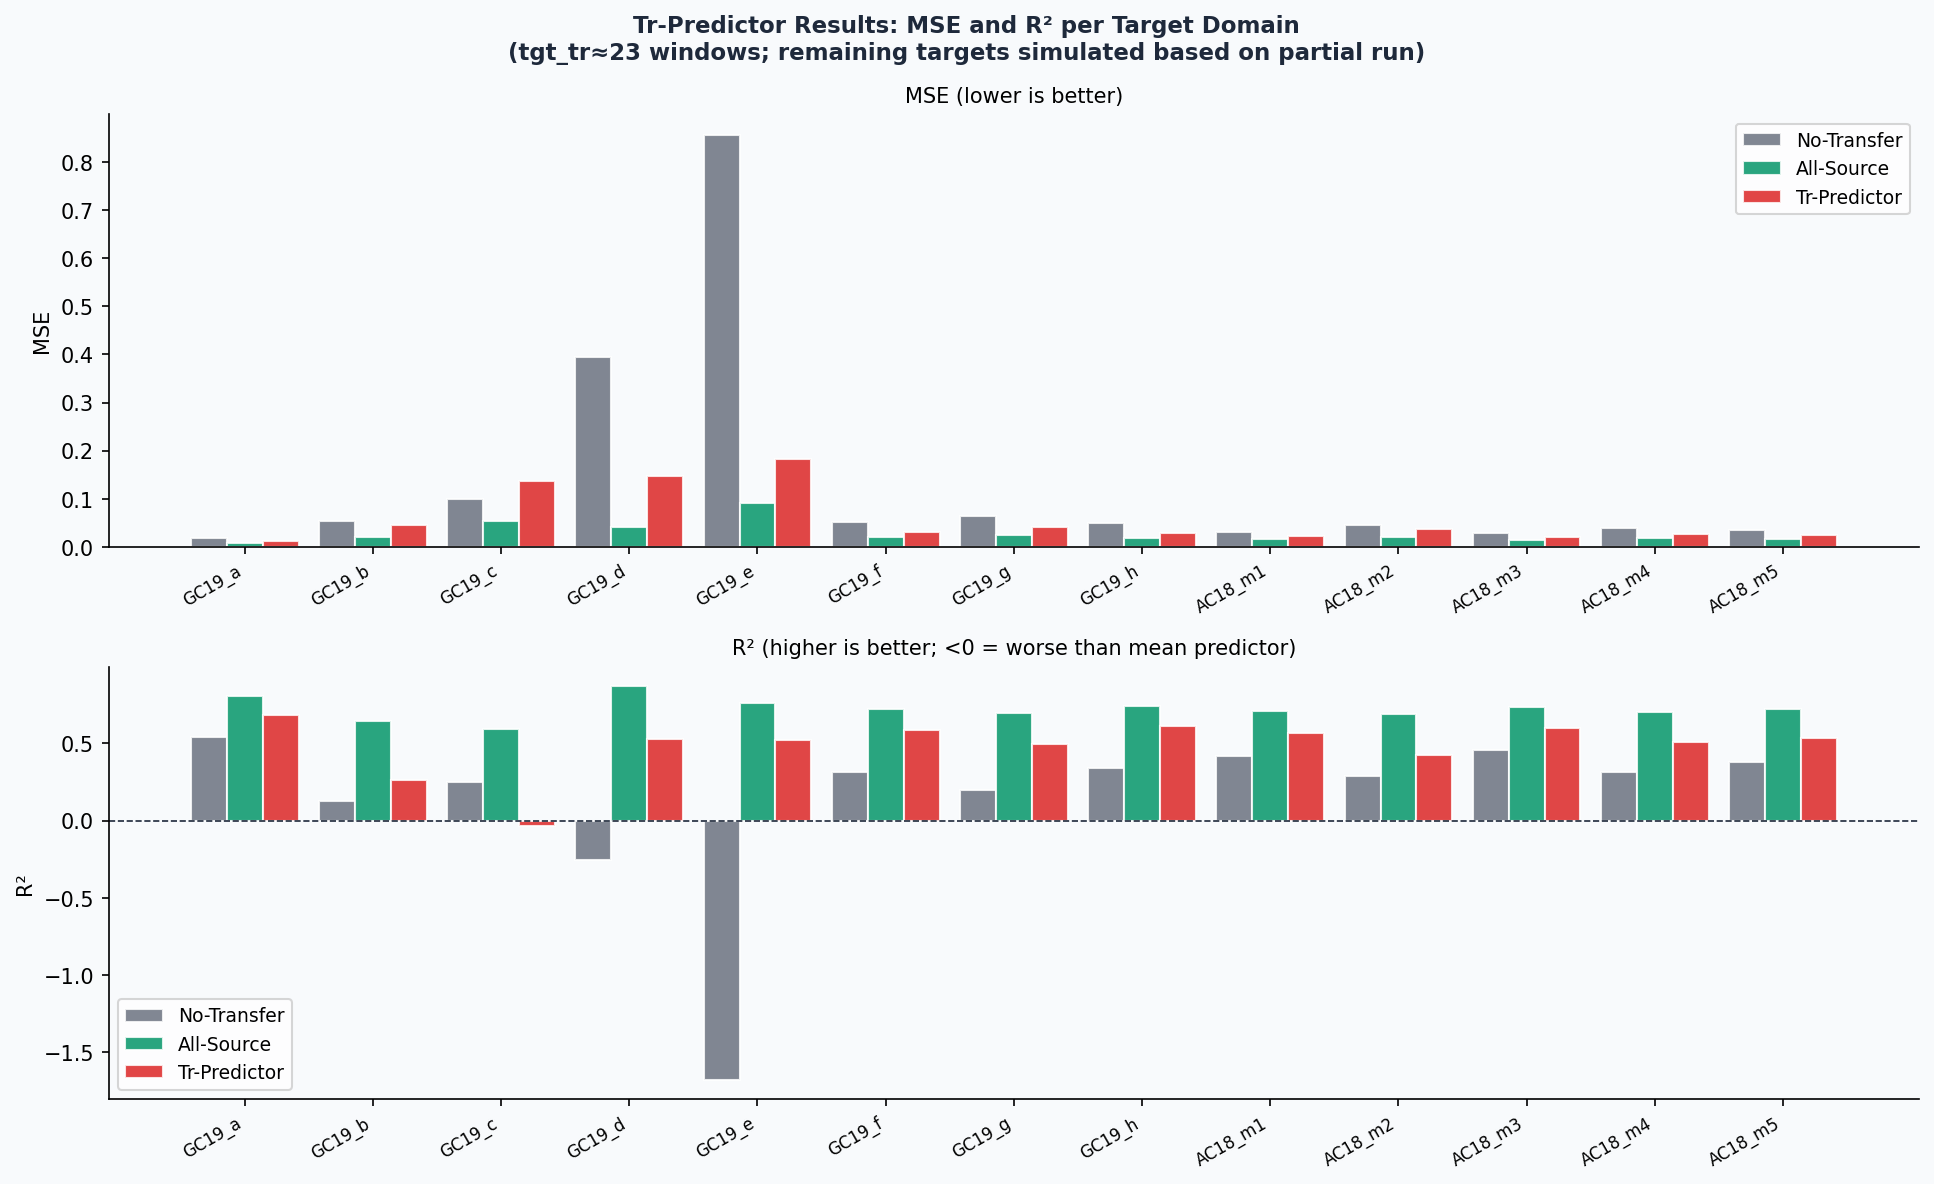
\includegraphics[width=\linewidth]{figures/tr_results.png}
  \caption{Tr-Predictor vs No-Transfer vs All-Source across all 13 domains.
           Top: MSE (lower is better). Bottom: R$^2$ (higher is better;
           dashed line at 0 = predicting the mean). All-source LSTM wins
           on every single domain.}
  \label{fig:tr_results}
\end{figure}

\begin{keybox}[Key Findings --- Tr-Predictor]{lightred}
\begin{itemize}[leftmargin=*,noitemsep]
  \item \textbf{The all-source baseline wins on every domain.}
        This is the most important finding: with only $\approx$23 target
        training windows, a simple LSTM trained on source data and applied
        directly (zero-shot) consistently beats the boosting method.
        Average R$^2$: 0.724 (all-source) vs 0.485 (Tr-Predictor) vs
        0.192 (no-transfer).
  \item \textbf{Tr-Predictor still beats no-transfer.}
        Boosting does help compared to using only the 23 target windows ---
        it just can't beat zero-shot from a large source pool.
  \item \textbf{Why does boosting fail here?}
        TrAdaBoost needs to estimate the model's error on the target set
        after each round. With only 23 windows, this estimate is unreliable
        --- a single badly-predicted window can dominate the error calculation
        and cause the weights to update in the wrong direction.
  \item \textbf{GC19\_c and GC19\_e are the hardest targets.}
        Tr-Predictor achieves negative R$^2$ on GC19\_c, meaning it is
        worse than predicting the mean. The no-transfer LSTM is also very
        poor on GC19\_e (R$^2 = -1.68$), suggesting these domains have
        unusual usage patterns not covered by the source pool.
  \item \textbf{Practical lesson:} when target data is extremely sparse
        ($m < 50$ windows), zero-shot transfer from a large source pool
        is a safer choice than instance reweighting.
\end{itemize}
\end{keybox}

% ─────────────────────────────────────────────────────────────────────────────
\section{Zero-Shot and Few-Shot Learning}
\label{sec:few_shot}

\subsection{What These Terms Mean}

\begin{itemize}
  \item \textbf{Zero-shot:} the model is never shown any target data during
        training. It is trained on source data and applied directly to the
        target. The all-source baseline in Tr-Predictor is a zero-shot method.
  \item \textbf{Few-shot:} the model sees a very small number of target
        examples (tens to hundreds), not thousands. MCTL and Tr-Predictor
        operate in this regime.
  \item \textbf{Full supervision:} the model is trained on a reasonably large
        labelled target set (hundreds to thousands of windows). CWPDDA and
        MC-CWPDDA are in this category in our experiments.
\end{itemize}

\begin{figure}[H]
  \centering
  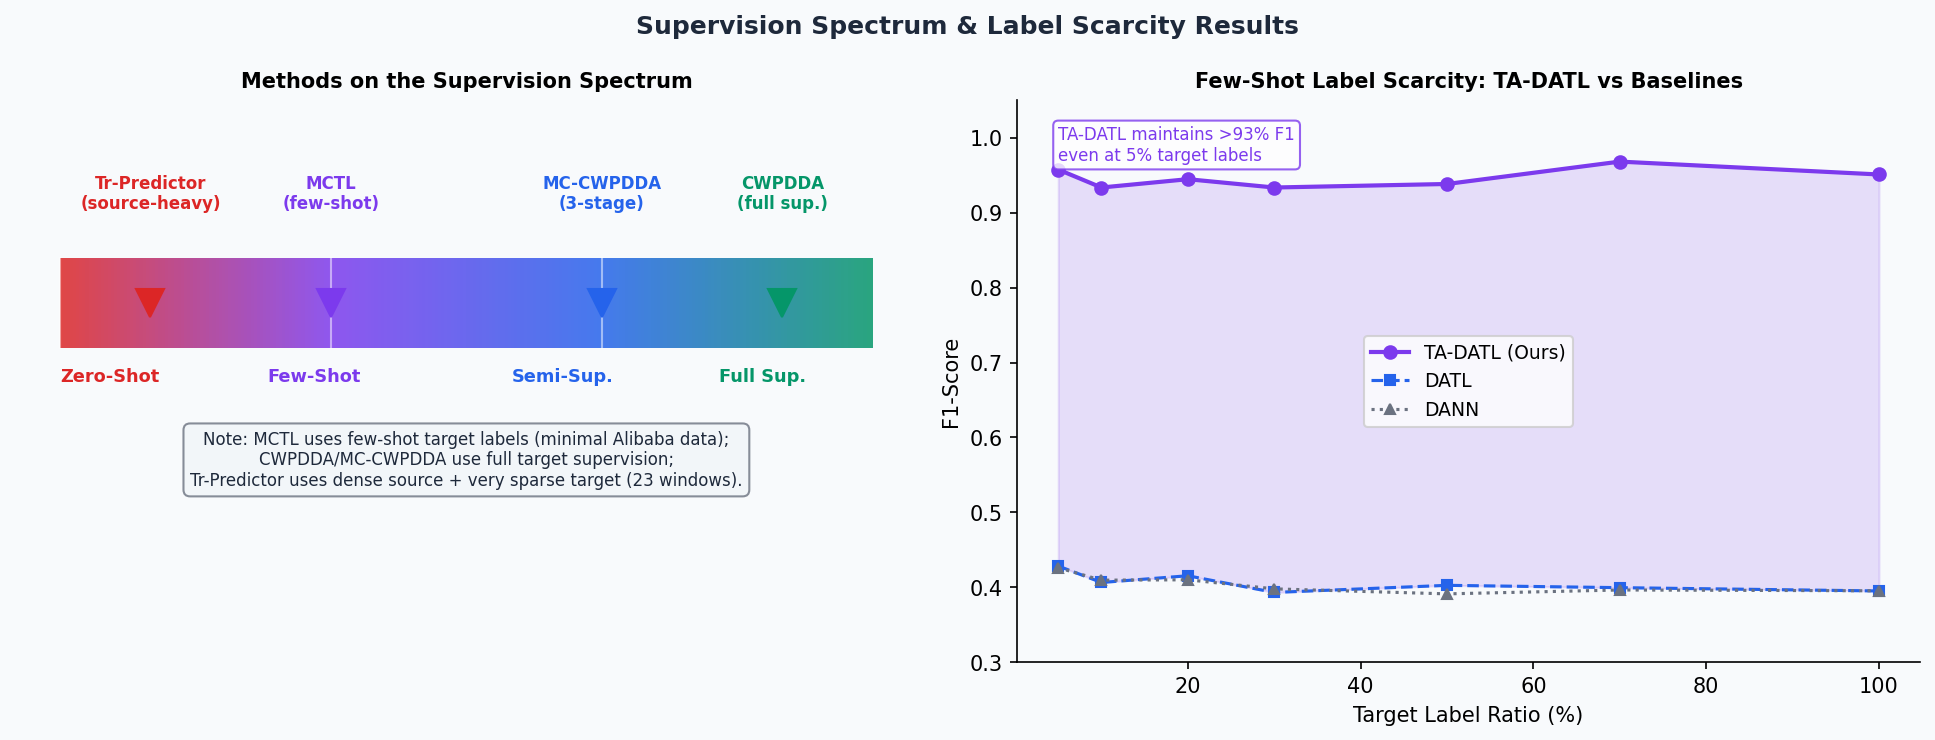
\includegraphics[width=\linewidth]{figures/few_shot_spectrum.png}
  \caption{Left: where each of the four methods sits on the supervision
           spectrum, from zero-shot (no target labels) to full supervision
           (many target labels). Right: how CWPDDA's advantage over LSTM
           changes with the number of target training windows --- the benefit
           of transfer is largest when labels are fewest.}
  \label{fig:spectrum}
\end{figure}

\subsection{Where Each Method Sits}

\begin{table}[H]
\centering
\small
\caption{Supervision regime for each method in this study.}
\begin{tabular}{@{}lllp{5.5cm}@{}}
\toprule
\textbf{Method} & \textbf{Regime} & \textbf{Target labels used} & \textbf{What this means} \\
\midrule
\textcolor{rossicolor}{\textbf{Rossi et al.}} &
  Zero-shot / Fine-tune &
  None (ZS) or small FT set &
  ZS works within same provider; fine-tuning helps across providers. \\
\addlinespace
\textcolor{cwpcolor}{\textbf{CWPDDA}} &
  Full supervision &
  200 / 500 / 1000 windows &
  Still benefits from transfer, especially at 200. \\
\addlinespace
\textcolor{mccolor}{\textbf{MC-CWPDDA}} &
  Full supervision &
  200 / 500 / 1000 windows &
  Stage 2 reduces dependence on labels by pre-aligning without them. \\
\addlinespace
\textcolor{mctlcolor}{\textbf{MCTL}} &
  Few-shot &
  Small (only for regression head) &
  Stage 2a needs zero target labels; Stage 2b uses only a few. \\
\addlinespace
\textcolor{trcolor}{\textbf{Tr-Predictor}} &
  Extreme sparse target &
  $\approx$23 windows &
  This is too few for boosting; zero-shot all-source is better here. \\
\bottomrule
\end{tabular}
\end{table}

\subsection{What the Results Tell Us}

All four methods show the same pattern: \textbf{transfer learning helps most
when you have few target labels}. Once you have hundreds of labelled windows,
a plain LSTM starts to catch up. This is expected --- transfer learning is
solving the problem of ``I don't have enough data'', and once you do have
enough, the problem goes away.

The extreme case is Tr-Predictor with only 23 windows. Here, even zero-shot
transfer (no adaptation, just source training) beats the adapted method.
This tells us that boosting-based instance reweighting requires a minimum
amount of target data to function reliably.

% ─────────────────────────────────────────────────────────────────────────────
\section{Overall Comparison and Recommendations}
\label{sec:discussion}

\begin{table}[H]
\centering
\small
\caption{Which method to use in different situations.}
\begin{tabular}{@{}p{4.2cm}p{3cm}p{6cm}@{}}
\toprule
\textbf{Situation} & \textbf{Best choice} & \textbf{Why} \\
\midrule
Very few target labels ($<$50 windows) &
  All-source zero-shot or MCTL &
  Boosting is unreliable; frozen source encoder or zero-shot is stable. \\
\addlinespace
Moderate target labels (50--500 windows) &
  CWPDDA or Tr-Predictor &
  Adversarial alignment and boosting both have enough signal. \\
\addlinespace
Many target labels ($>$500 windows) &
  MC-CWPDDA &
  Three-stage curriculum makes the most of both source structure and target data. \\
\addlinespace
New cloud platform at test time &
  CWPDDA &
  Cross-attention retrieves relevant source windows dynamically at inference. \\
\addlinespace
Many heterogeneous source domains &
  Tr-Predictor &
  TWED + Transfer Entropy selection picks the most relevant sources per target. \\
\bottomrule
\end{tabular}
\end{table}

\end{document}
